The quality of the as-bought h-BN on copper foils\cite{_graphene_2014} is examined in XPS.
%%%%%%%%%%%%%%%%%%%%%%%%%%%% make it better looking? %%%%%%%%%%%%%%%%%%%%%%%%%%%%%%%%%%%%%
\begin{figure}
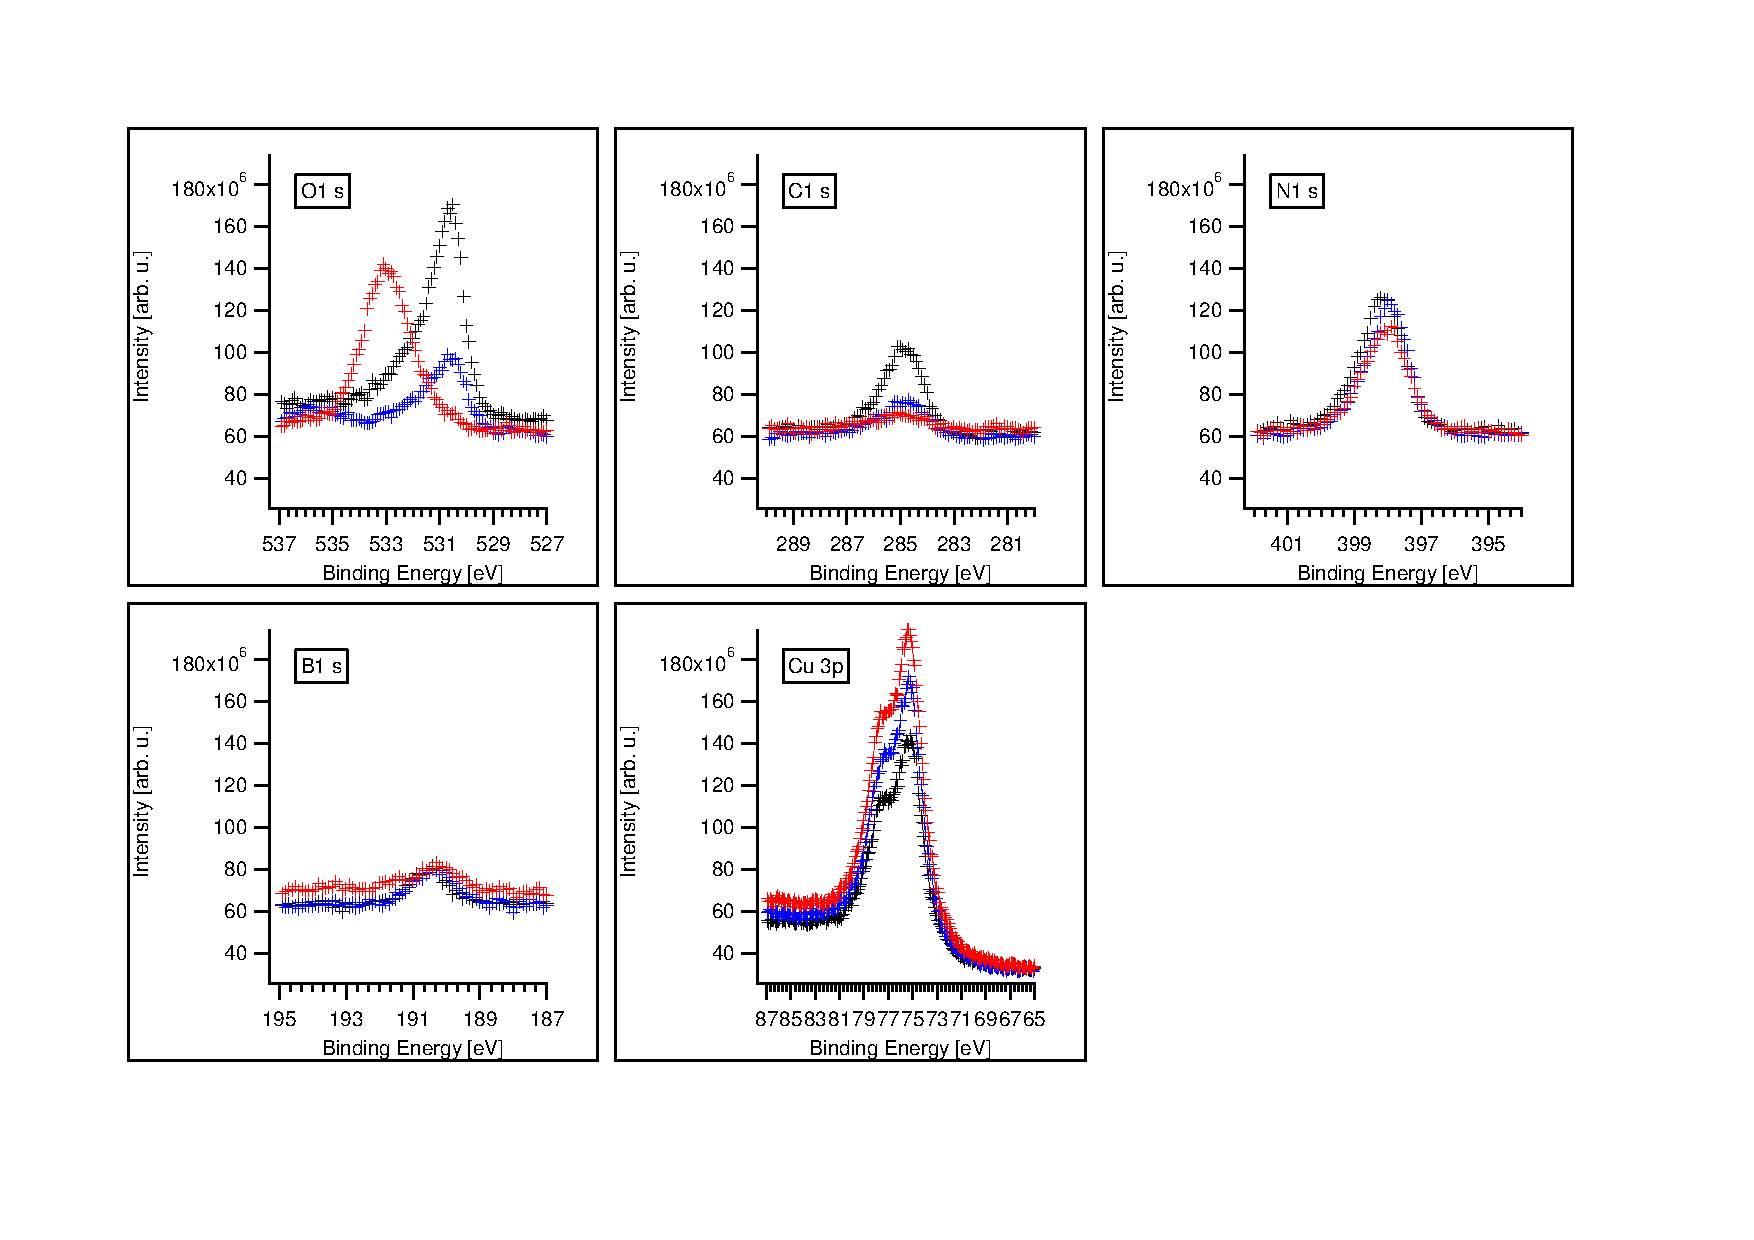
\includegraphics[angle=90,width=1.2\textwidth]{./images/XPS-spectra-as-bought.pdf}
\caption{XPS spectra of as-bought h-BN/Cu-foil sample\cite{_graphene_2014}}
\end{figure}
%%%%%%%%%%%%%%%%%%%%%%%%%%%% 
The XPS spectra shows contribution of different atomic species. There are peaks for the O-atoms (1s: \SIrange{529}{535}{\eV})), C-atoms (1s $\approx \SI{285}{\eV}$), N-atoms (1s $\approx \SI{398}{\eV}$), B-atoms (1s $\approx \SI{190}{\eV}$) and Cu-atoms ($3p_{1/2,3/2}$: \SIrange{70}{80}{\eV})). One would expect the shape of the 1s-peaks to be singlet-like (one peak, gauss shaped) and the 3p-peak to be a doublet (two close lying peaks with area-ratio 1/2:3/2=1:2).

\paragraph{O1s}
Position varies with temperature. The signal at room temperature(black) stems from adsorbed water and CO. These desorp with increasing temperature(blue). When going to higher temperatures(red) this peak increases again and shifts to higher binding energies. Not present in self-grown h-BN (figure \ref{fig:xps-self-grown})

\paragraph{C1s}
The C1s Peak decreases with increasing temperature and retains its position. This has the same  reason as for the O1s peak (desorption of CO due to the heating). Some of the carbon remains on the surface - even at temperatures as high as \SI{970}{\K}.

\paragraph{N1s/B1s}
The nitrogen/boron peaks show some temperature related changes. There is little change upon annealing to \SI{630}{\K}, both peaks shrink, but stay almost constant in their position in binding energy (sightly shifted to lower binding energies by about \SI{0.2}{\eV}). Position is [N1s: \SI{398.1}{\eV} | B1s: \SI{190.2}{\eV}]

\paragraph{Cu3p}
The copper peak exhibits an increase in area when increasing the temperature. This is because some of the water and CO adsorbate desorb and more and more copper is contributing to the signal. This peak is a doublet, so both signals come from the same chemical copper surrounding.


The $Cu(OH)_2$ O1s peak is expected to be at \SIrange{531.3}{531.7}{\eV}\cite{deroubaix_x-ray_1992} which may explain the shoulder of the O1s peak to higher binding energies (O1s metal: \SI{531}{\eV}). Nitrates ($NO_3$) have binding energies in the range from \SIrange{532.5}{533.5}{\eV}\cite[45]{wanger_handbook_1979}. This would imply either an replacement of nitrogen with oxygen, or some kind of oxygen on top or below the nitrogen in the BN. As proven by Simonov et al. in \cite{simonov_controllable_2012} the (!atomic!) oxygen tends to replace the nitrogen in the h-BN/Ir(111) system when it is annealed to \SI{600}{\degreeCelsius} (compare figure eight therein). Thus it forms $B_{x}N_{y}O_{1-x-y}$ over-layers. The longer the oxidation time the higher the amount of replaced nitrogen (figure two therein). If this effect is responsible for the O1s peak at high temperatures is questionable, since the oxygen has to be cracked somehow - where no process can be thought of (no catalytic cracking at metal surface possible - full ML, thermal energy to low to reach binding energies of $O_2$ (no citation here, nothing found - just a guess)).
%%%%%%%%%%%%%%%%%%%%%%%%%%%%%%%%%%%%%%%%%%%%%%%%%%%%%%%%%%%%%%%%%%%%%%%%%%%%%%%%%%%%
% % This refers to the analysis of the series with unknown temperature reading
% The Cu/B/N-peaks have the expected shape, representing the singlet/doublet structure of the atoms. The O1s peak look different though. The peak should exhibit a single peak, while the recorded spectrum showd a clear double-peak structure. It consists of the expected O1s core level, shifed to lower binding energies and a second contribution, shifted to higher binding energies.
% 
% There are different species expected to be present on the unprepared sample surface. These are namely $CO$/$CO_2$, $CuO$/$Cu_2O$ and $H_2O$. They are availble to the surface due to storage at athmospheric conditions. While hydroxy- compounds shift the O1s-peak to higher BE's, metal oxydes push it to lower BE's \cite{wanger_handbook_1979}. The $H_2O$ peak is expected to be at $\approx \SI{533}{\eV}$ (ausm Kopf - Quelle willi H2O/St($\approx 534$), H2O/Ir (531,9)).
% 
% A contribution of $B_xO_x$/$N_xO_x$ species would result in a broadening of B/N-peaks ($>\SI{191,5}{\eV}$ \cite[6386]{kidambi_observing_2013}) and an increase in the O-signal \cite[6386]{kidambi_observing_2013}. A typical shape of the O-peak for Cu (metal), $CU_2O$ and $CuO$ can be seen in \cite[41]{deroubaix_x-ray_1992}.
%%%%%%%%%%%%%%%%%%%%%%%%%%%%%%%%%%%%%%%%%%%%%%%%%%%%%%%%%%%%%%%%%%%%%%%%%%%%%%%%%%%%
\paragraph{An exchange of O with B or N would be easily visible in XPS (due to changed N/B surroundings. Not sure if the signal of oxygen is large enough for that. Check DATA - confirm maybe}